\documentclass[11pt]{article}

\usepackage[margin=1in]{geometry}
\usepackage{amsmath, amssymb, amsthm, mathtools, bm}
\usepackage{graphicx}
\usepackage{algorithm}
\usepackage{float}
\usepackage{algpseudocode}
\usepackage{hyperref}
\usepackage{listings}
\usepackage{xcolor}
\usepackage{booktabs}
\usepackage{multirow}
\usepackage{tikz}
\usetikzlibrary{shapes,arrows,positioning,calc}

\lstdefinestyle{python}{
  language=Python,
  basicstyle=\ttfamily\small,
  keywordstyle=\bfseries\color{blue},
  commentstyle=\itshape\color{green!60!black},
  stringstyle=\color{red},
  showstringspaces=false,
  frame=single,
  breaklines=true,
  numbers=left,
  numberstyle=\tiny\color{gray}
}

\title{TurtleBot Interceptor: Complete System Architecture and Algorithms\\
\large Comprehensive Technical Documentation for Presentation}
\author{Tim, Gabe, Thomas, Ryan, Kush}
\date{}

\begin{document}
\maketitle

\tableofcontents
\newpage

\section{System Overview}

The TurtleBot Interceptor system is a complete ROS2-based autonomous interception system that combines multiple sensing modalities, state estimation, mapping, and optimal control to intercept a moving target robot in unknown, cluttered environments.

\subsection{High-Level Architecture}

The system consists of four main layers:

\begin{enumerate}
    \item \textbf{Sensor Layer}: LIDAR, Camera, IMU, Magnetometer, Wheel Encoders
    \item \textbf{State Estimation Layer}: \textbf{EKF for robot pose} (100 Hz), Target Estimator for target pose
    \item \textbf{Mapping Layer}: Cartographer SLAM + Fast Local Grid for environment mapping
    \item \textbf{Control Layer}: MPC for optimal interception with obstacle avoidance
\end{enumerate}

\textbf{Key Design Decision:} The system uses \textbf{EKF for robot localization} instead of MCL because:
\begin{itemize}
    \item Higher update rate (100 Hz vs 10 Hz) for smooth control
    \item Lower computational cost
    \item Magnetometer fusion prevents heading drift
    \item Multi-sensor fusion (IMU + mag + encoders) provides robust state
\end{itemize}

MCL is available for simulation and research but is \textbf{not used in hardware deployment}.

\section{Complete Node System Architecture}

\subsection{Node Graph}

The complete system consists of the following ROS2 nodes:

\begin{table}[H]
\centering
\caption{Complete Node List}
\begin{tabular}{|l|l|l|}
\hline
\textbf{Node Name} & \textbf{Executable} & \textbf{Purpose} \\
\hline
\texttt{ekf\_pose\_estimator} & \texttt{ekf\_pose\_estimator} & Robot state estimation (EKF) \\
\texttt{cartographer\_node} & \texttt{cartographer\_node} & SLAM mapping (external) \\
\texttt{fast\_local\_grid} & \texttt{fast\_local\_grid} & Fast local occupancy grid (5-10 Hz) \\
\texttt{fast\_local\_grid\_target} & \texttt{fast\_local\_grid\_target} & Target-side fast local grid \\
\texttt{camera\_cone\_detector} & \texttt{camera\_cone\_detector} & Vision-based cone detection \\
\texttt{target\_est\_node} & \texttt{target\_est\_node} & Target pose estimation \\
\texttt{target\_ekf\_node} & \texttt{target\_ekf\_node} & Target velocity tracking \\
\texttt{mpc\_node} & \texttt{mpc\_node} & Model Predictive Control \\
\texttt{navigation\_visualizer} & \texttt{navigation\_visualizer\_node} & RViz visualization \\
\texttt{mcl\_node} & \texttt{mcl\_node} & MCL localization (optional, simulation only) \\
\hline
\end{tabular}
\end{table}

\subsection{Complete Topic Graph}

\begin{table}[H]
\centering
\caption{Complete Topic List}
\begin{tabular}{|l|l|l|l|}
\hline
\textbf{Topic} & \textbf{Type} & \textbf{Publisher} & \textbf{Subscriber} \\
\hline
\hline
\multicolumn{4}{|c|}{\textbf{Sensor Topics}} \\
\hline
\texttt{/scan} & \texttt{LaserScan} & LIDAR driver & Cartographer, MPC \\
\texttt{/camera/image\_raw} & \texttt{Image} & Camera driver & Camera detector \\
\texttt{/imu} & \texttt{Imu} & Robot driver & EKF \\
\texttt{/magnetic\_field} & \texttt{MagneticField} & Robot driver & EKF \\
\texttt{/odom} & \texttt{Odometry} & Robot driver & EKF, Cartographer \\
\hline
\multicolumn{4}{|c|}{\textbf{State Estimation Topics}} \\
\hline
\texttt{/amcl\_pose} & \texttt{PoseWithCovarianceStamped} & EKF & MPC, Cartographer \\
\texttt{/odom\_ekf} & \texttt{Odometry} & EKF & Cartographer \\
\texttt{/target\_est} & \texttt{PoseWithCovarianceStamped} & Target estimator & MPC \\
\texttt{/target\_pose\_measurement} & \texttt{PoseStamped} & Target estimator & Target EKF \\
\texttt{/target\_estimate} & \texttt{PoseWithCovarianceStamped} & Target EKF & MPC \\
\hline
\multicolumn{4}{|c|}{\textbf{Mapping Topics}} \\
\hline
\texttt{/map} & \texttt{OccupancyGrid} & Cartographer & Fast Local Grid, MPC \\
\texttt{/local\_map} & \texttt{OccupancyGrid} & Fast Local Grid & MPC \\
\texttt{/local\_map\_target} & \texttt{OccupancyGrid} & Fast Local Grid Target & Target Estimator \\
\hline
\multicolumn{4}{|c|}{\textbf{Vision Topics}} \\
\hline
\texttt{/camera\_cone\_positions} & \texttt{PointStamped} & Camera detector & MPC \\
\texttt{/camera\_target\_positions} & \texttt{PointStamped} & Camera detector & Target estimator \\
\texttt{/camera\_cones} & \texttt{MarkerArray} & Camera detector & RViz \\
\texttt{/camera\_target\_markers} & \texttt{MarkerArray} & Camera detector & RViz \\
\hline
\multicolumn{4}{|c|}{\textbf{Control Topics}} \\
\hline
\texttt{/cmd\_vel} & \texttt{Twist} & MPC & Robot driver \\
\hline
\end{tabular}
\end{table}

\subsection{Data Flow Diagram}

\begin{figure}[H]
\centering
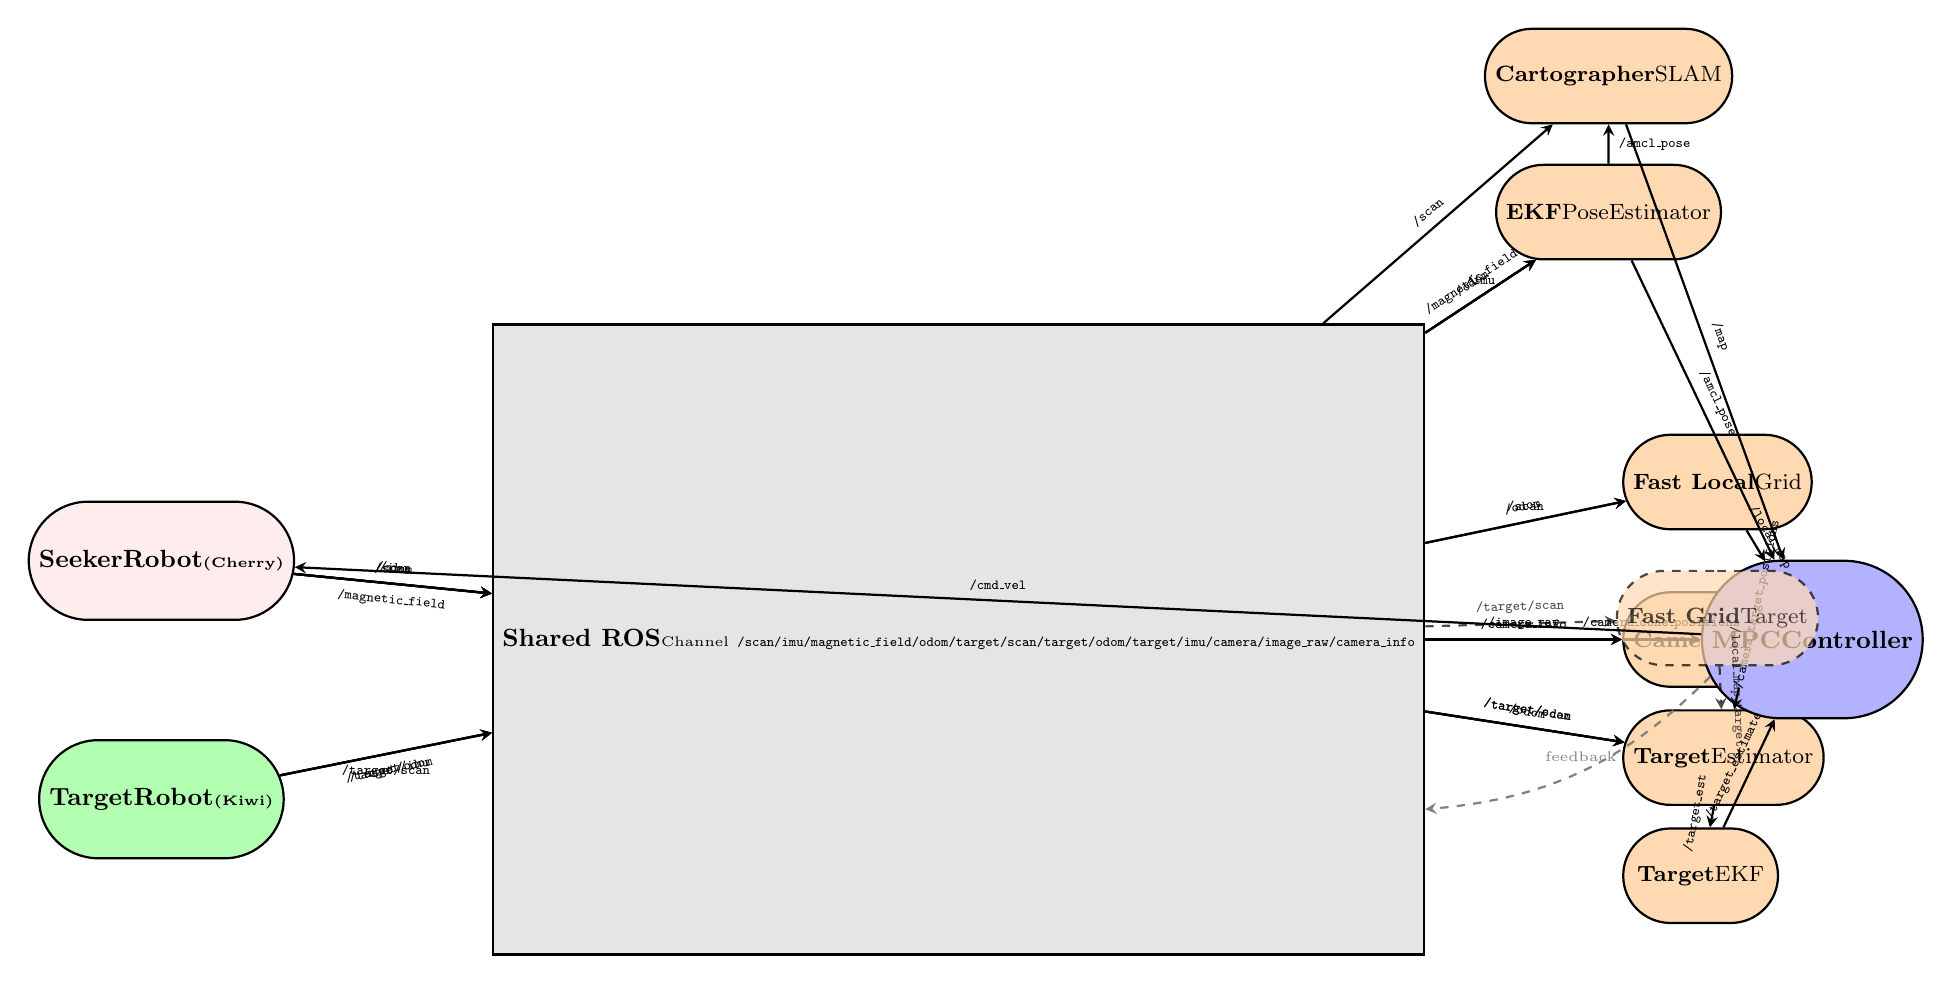
\begin{tikzpicture}[
    node distance=1.5cm and 2.5cm,
    robot/.style={rounded rectangle, fill=pink!30, draw=black, thick, minimum width=2.5cm, minimum height=1.5cm, text centered, font=\small\bfseries},
    target/.style={rounded rectangle, fill=green!30, draw=black, thick, minimum width=2.5cm, minimum height=1.5cm, text centered, font=\small\bfseries},
    channel/.style={rectangle, fill=gray!20, draw=black, thick, minimum width=3cm, minimum height=8cm, text centered, font=\small},
    process/.style={rounded rectangle, fill=orange!30, draw=black, thick, minimum width=2.2cm, minimum height=1.2cm, text centered, font=\footnotesize},
    mpc/.style={rounded rectangle, fill=blue!30, draw=black, thick, minimum width=2.5cm, minimum height=2cm, text centered, font=\small\bfseries},
    arrow/.style={->, >=stealth, thick},
    label/.style={font=\tiny}
]

    % Robots (left side)
    \node[robot] (seeker) {Seeker\\Robot\\{\tiny (Cherry)}};
    \node[target, below=of seeker] (target_robot) {Target\\Robot\\{\tiny (Kiwi)}};
    
    % Shared ROS Channel (center)
    \node[channel, right=of seeker, yshift=-1cm] (channel) {\textbf{Shared ROS}\\{\tiny Channel}\\[0.2cm]
        \tiny\texttt{/scan}\\
        \tiny\texttt{/imu}\\
        \tiny\texttt{/magnetic\_field}\\
        \tiny\texttt{/odom}\\
        \tiny\texttt{/target/scan}\\
        \tiny\texttt{/target/odom}\\
        \tiny\texttt{/target/imu}\\
        \tiny\texttt{/camera/image\_raw}\\
        \tiny\texttt{/camera\_info}
    };
    
    % Processing nodes (right of channel)
    \node[process, above right=0.8cm and 1.5cm of channel] (ekf_seeker) {\textbf{EKF}\\Pose\\Estimator};
    \node[process, right=of channel, yshift=2cm] (fast_grid) {\textbf{Fast Local}\\Grid};
    \node[process, right=of channel, yshift=0cm] (camera) {\textbf{Camera}\\Cone\\Detector};
    \node[process, right=of channel, yshift=-1.5cm] (target_est) {\textbf{Target}\\Estimator};
    \node[process, right=of channel, yshift=-3cm] (target_ekf) {\textbf{Target}\\EKF};
    
    % Cartographer (above EKF)
    \node[process, above=0.5cm of ekf_seeker] (cartographer) {\textbf{Cartographer}\\SLAM};
    
    % MPC (rightmost)
    \node[mpc, right=3.5cm of channel] (mpc) {\textbf{MPC}\\Controller};
    
    % Robot to Channel arrows
    \draw[arrow] (seeker) -- node[label, above] {\tiny\texttt{/scan}} (channel);
    \draw[arrow] (seeker) -- node[label, above, sloped] {\tiny\texttt{/imu}} (channel);
    \draw[arrow] (seeker) -- node[label, above, sloped] {\tiny\texttt{/odom}} (channel);
    \draw[arrow] (seeker) -- node[label, below, sloped] {\tiny\texttt{/magnetic\_field}} (channel);
    
    \draw[arrow] (target_robot) -- node[label, below] {\tiny\texttt{/target/scan}} (channel);
    \draw[arrow] (target_robot) -- node[label, below, sloped] {\tiny\texttt{/target/odom}} (channel);
    \draw[arrow] (target_robot) -- node[label, below, sloped] {\tiny\texttt{/target/imu}} (channel);
    
    % Channel to processing nodes
    \draw[arrow] (channel) -- node[label, above] {\tiny\texttt{/imu}} (ekf_seeker);
    \draw[arrow] (channel) -- node[label, above, sloped] {\tiny\texttt{/magnetic\_field}} (ekf_seeker);
    \draw[arrow] (channel) -- node[label, above, sloped] {\tiny\texttt{/odom}} (ekf_seeker);
    
    \draw[arrow] (channel) -- node[label, above] {\tiny\texttt{/scan}} (fast_grid);
    \draw[arrow] (channel) -- node[label, above, sloped] {\tiny\texttt{/odom}} (fast_grid);
    
    \draw[arrow] (channel) -- node[label, above] {\tiny\texttt{/image\_raw}} (camera);
    \draw[arrow] (channel) -- node[label, above, sloped] {\tiny\texttt{/camera\_info}} (camera);
    
    \draw[arrow] (channel) -- node[label, above, sloped] {\tiny\texttt{/target/scan}} (target_est);
    \draw[arrow] (channel) -- node[label, above, sloped] {\tiny\texttt{/odom}} (target_est);
    \draw[arrow] (channel) -- node[label, above, sloped] {\tiny\texttt{/target/odom}} (target_est);
    
    % Processing nodes to MPC
    \draw[arrow] (ekf_seeker) -- node[label, above, sloped] {\tiny\texttt{/amcl\_pose}} (mpc);
    \draw[arrow] (fast_grid) -- node[label, above, sloped] {\tiny\texttt{/local\_map}} (mpc);
    \draw[arrow] (camera) -- node[label, above, sloped] {\tiny\texttt{/camera\_cone\_positions}} (mpc);
    \draw[arrow] (target_est) -- node[label, above, sloped] {\tiny\texttt{/target\_est}} (target_ekf);
    \draw[arrow] (target_ekf) -- node[label, above, sloped] {\tiny\texttt{/target\_estimate}} (mpc);
    
    % Cartographer connections
    \draw[arrow] (channel) -- node[label, above, sloped] {\tiny\texttt{/scan}} (cartographer);
    \draw[arrow] (ekf_seeker) -- node[label, right] {\tiny\texttt{/amcl\_pose}} (cartographer);
    \draw[arrow] (cartographer) -- node[label, above, sloped] {\tiny\texttt{/map}} (mpc);
    
    % Target estimator to target EKF
    \draw[arrow] (camera) -- node[label, right, sloped] {\tiny\texttt{/camera\_target\_positions}} (target_est);
    
    % Fast Local Grid Target (optional, shown as dashed)
    \node[process, below=0.5cm of fast_grid, dashed, opacity=0.7] (fast_grid_target) {\textbf{Fast Grid}\\Target};
    \draw[arrow, dashed, opacity=0.7] (channel) -- node[label, above, sloped] {\tiny\texttt{/target/scan}} (fast_grid_target);
    \draw[arrow, dashed, opacity=0.7] (fast_grid_target) -- node[label, above, sloped] {\tiny\texttt{/local\_map\_target}} (target_est);
    
    % MPC back to robot
    \draw[arrow, thick] (mpc) -- node[label, above] {\tiny\texttt{/cmd\_vel}} (seeker);
    
    % Feedback loops (curved)
    \draw[arrow, bend left=20, dashed, gray] (mpc) to node[label, above] {\tiny feedback} (channel);
    
\end{tikzpicture}
\caption{Complete ROS2 System Architecture: Data flow from Seeker and Target robots through Shared ROS Channel to processing nodes and MPC controller.}
\label{fig:ros_architecture}
\end{figure}

\section{Node-by-Node Detailed Description}

\subsection{EKF Pose Estimator Node}

\textbf{Purpose:} Fuse IMU, magnetometer, and wheel encoders to provide high-rate, accurate robot pose estimation.

\textbf{State Vector:}
\[
\mathbf{x} = \begin{bmatrix} x \\ y \\ \theta \\ v_x \\ v_y \\ \omega \end{bmatrix}
\]

\textbf{Subscriptions:}
\begin{itemize}
    \item \texttt{/imu} (sensor\_msgs/Imu): Accelerometer and gyroscope data
    \item \texttt{/magnetic\_field} (sensor\_msgs/MagneticField): Magnetometer data
    \item \texttt{/odom} (nav\_msgs/Odometry): Wheel encoder velocities
\end{itemize}

\textbf{Publications:}
\begin{itemize}
    \item \texttt{/amcl\_pose} (geometry\_msgs/PoseWithCovarianceStamped): Robot pose estimate at 100 Hz
    \item \texttt{/odom\_ekf} (nav\_msgs/Odometry): Refined odometry for Cartographer
\end{itemize}

\textbf{Algorithm:}

\begin{algorithm}[H]
\caption{Extended Kalman Filter}
\begin{algorithmic}[1]
\State Initialize: $\mathbf{x}_0$, $\mathbf{P}_0$
\State Calibrate magnetometer (first 10 seconds)
\Loop{Every IMU update (100 Hz)}
    \State \textbf{Prediction:}
    \State $\mathbf{x}_{k|k-1} = f(\mathbf{x}_{k-1|k-1}, \mathbf{u}_{k-1})$
    \State $\mathbf{P}_{k|k-1} = \mathbf{F}_k \mathbf{P}_{k-1|k-1} \mathbf{F}_k^T + \mathbf{Q}_k$
    \State \textbf{Update (if measurement available):}
    \State $\mathbf{K}_k = \mathbf{P}_{k|k-1} \mathbf{H}_k^T (\mathbf{H}_k \mathbf{P}_{k|k-1} \mathbf{H}_k^T + \mathbf{R}_k)^{-1}$
    \State $\mathbf{x}_{k|k} = \mathbf{x}_{k|k-1} + \mathbf{K}_k (\mathbf{z}_k - h(\mathbf{x}_{k|k-1}))$
    \State $\mathbf{P}_{k|k} = (\mathbf{I} - \mathbf{K}_k \mathbf{H}_k) \mathbf{P}_{k|k-1}$
    \State Publish $\mathbf{x}_{k|k}$, $\mathbf{P}_{k|k}$
\EndLoop
\end{algorithmic}
\end{algorithm}

\textbf{Process Model:}
\begin{align}
x_{k+1} &= x_k + \Delta t (v_{x,k} \cos\theta_k - v_{y,k} \sin\theta_k) \\
y_{k+1} &= y_k + \Delta t (v_{x,k} \sin\theta_k + v_{y,k} \cos\theta_k) \\
\theta_{k+1} &= \theta_k + \Delta t \cdot \omega_k \\
v_{x,k+1} &= v_{x,k} \quad \text{(updated by measurements)} \\
v_{y,k+1} &= v_{y,k} \quad \text{(updated by measurements)} \\
\omega_{k+1} &= \omega_k \quad \text{(updated by measurements)}
\end{align}

\textbf{Measurement Models:}

\textbf{IMU Gyroscope:}
\[
z_{\omega} = \omega + v_{\omega}, \quad v_{\omega} \sim \mathcal{N}(0, 0.01)
\]

\textbf{IMU Accelerometer (gravity-compensated):}
\[
\mathbf{a}_{\text{world}} = \mathbf{R}(\theta) \mathbf{a}_{\text{IMU}} - \mathbf{g}
\]
\[
\dot{v}_x = a_{x,\text{world}}, \quad \dot{v}_y = a_{y,\text{world}}
\]

\textbf{Magnetometer:}
\[
\theta_{\text{mag}} = \atan2(m_y, m_x) - \theta_{\text{offset}}
\]
where $\theta_{\text{offset}}$ is calibrated at startup by rotating robot 360$^\circ$.

\textbf{Wheel Encoders:}
\[
z_{v_x} = v_x + v_{v_x}, \quad z_{v_y} = v_y + v_{v_y}, \quad z_{\omega} = \omega + v_{\omega}
\]

\subsection{Cartographer SLAM Node}

\textbf{Purpose:} Build persistent, high-resolution occupancy grid map of the environment.

\textbf{Subscriptions:}
\begin{itemize}
    \item \texttt{/scan} (sensor\_msgs/LaserScan): LIDAR data
    \item \texttt{/odom\_ekf} (nav\_msgs/Odometry): EKF odometry (constraint)
\end{itemize}

\textbf{Publications:}
\begin{itemize}
    \item \texttt{/map} (nav\_msgs/OccupancyGrid): 2 cm resolution occupancy grid at 1-2 Hz
\end{itemize}

\textbf{Key Features:}
\begin{itemize}
    \item Sub-mapping for efficiency
    \item Loop closure detection
    \item Scan matching for fine alignment
    \item Persistent obstacles (doesn't clear static objects)
\end{itemize}

\subsection{Fast Local Grid Node}

\textbf{Purpose:} High-speed local occupancy grid that updates at LIDAR rate (5-10 Hz) for dynamic navigation. Runs \textbf{alongside} Cartographer to provide immediate obstacle awareness.

\textbf{Key Difference from Cartographer:}
\begin{itemize}
    \item \textbf{Cartographer}: Global map, slow (1-2 Hz), accurate, persistent
    \item \textbf{Fast Local Grid}: Local map, fast (5-10 Hz), immediate, dynamic
\end{itemize}

\textbf{Subscriptions:}
\begin{itemize}
    \item \texttt{/scan} (sensor\_msgs/LaserScan): LIDAR data
    \item \texttt{/amcl\_pose} (geometry\_msgs/PoseWithCovarianceStamped): Robot pose
    \item \texttt{/map} (nav\_msgs/OccupancyGrid): Cartographer's global map (used as prior)
\end{itemize}

\textbf{Publications:}
\begin{itemize}
    \item \texttt{/local\_map} (nav\_msgs/OccupancyGrid): 5m $\times$ 5m robot-centric grid at 10 Hz
\end{itemize}

\textbf{Grid Parameters:}
\begin{itemize}
    \item Size: 5 m $\times$ 5 m (robot-centric window)
    \item Resolution: 5 cm (same as Cartographer)
    \item Grid dimensions: 100 $\times$ 100 cells
    \item Update rate: 10 Hz (publishes), 5-10 Hz (updates from LIDAR)
\end{itemize}

\textbf{Algorithm:}

\begin{algorithm}[H]
\caption{Fast Local Grid with World-Frame Storage}
\begin{algorithmic}[1]
\State Initialize: $\text{world\_obstacles} = \{\}$ (dictionary in world coordinates)
\State Initialize grid from Cartographer's global map (Bayesian prior)
\Loop{Every LIDAR scan}
    \State Decay existing obstacles: $\text{world\_obstacles}[key] \gets \text{world\_obstacles}[key] \times 0.95$
    \State Remove weak obstacles: if $|\text{world\_obstacles}[key]| < 0.5$, delete
    \For{each LIDAR beam $r_j$ at angle $\phi_j$}
        \State Compute ray endpoint in world frame:
            \State $\theta_{\text{world}} = \theta_{\text{robot}} + \phi_j + \theta_{\text{offset}}$
            \State $x_{\text{end}} = x_{\text{robot}} + r_j \cos(\theta_{\text{world}})$
            \State $y_{\text{end}} = y_{\text{robot}} + r_j \sin(\theta_{\text{world}})$
        \If{$r_j < r_{\max} \times 0.95$} \Comment{Hit obstacle}
            \State $key = \text{discretize}(x_{\text{end}}, y_{\text{end}})$
            \State $\text{world\_obstacles}[key] \gets \text{world\_obstacles}[key] + l_{\text{occ}}$
        \EndIf
        \State Mark free space along ray (sample every 10 cm):
            \For{$t = 0.1$ to $r_j$ step $0.1$}
                \State $x_{\text{free}} = x_{\text{robot}} + t \cos(\theta_{\text{world}})$
                \State $y_{\text{free}} = y_{\text{robot}} + t \sin(\theta_{\text{world}})$
                \State $key = \text{discretize}(x_{\text{free}}, y_{\text{free}})$
                \State $\text{world\_obstacles}[key] \gets \text{world\_obstacles}[key] + l_{\text{free}}$
            \EndFor
    \EndFor
    \State \textbf{Regenerate robot-centric grid:}
        \State Clear grid
        \State For each obstacle in world\_obstacles:
            \State If obstacle is within 5m $\times$ 5m window around robot:
                \State Project to robot-centric grid coordinates
                \State Store log-odds value
    \State Publish \texttt{/local\_map}
\EndLoop
\end{algorithmic}
\end{algorithm}

\textbf{Key Innovation: World-Frame Storage}

Unlike traditional robot-centric grids that lose obstacles when the robot moves, this system stores obstacles in \textbf{world coordinates}:

\begin{itemize}
    \item Obstacles stored as: $\{(x_{\text{world}}, y_{\text{world}}): \text{log\_odds}\}$
    \item Grid regenerated each update from world obstacles
    \item Obstacles persist as robot moves (don't disappear)
    \item Grid origin moves with robot but obstacles stay in world frame
\end{itemize}

\textbf{Log-Odds Parameters:}

\begin{align}
l_{\text{occ}} &= 2.0 \quad \text{(strong occupied evidence)} \\
l_{\text{free}} &= -0.4 \quad \text{(weak free evidence)} \\
l_{\min} &= -5.0 \\
l_{\max} &= 10.0
\end{align}

\textbf{Bayesian Fusion with Cartographer:}

The fast local grid uses Cartographer's global map as a prior:

\begin{enumerate}
    \item On startup: Import obstacles from Cartographer's \texttt{/map} within 10 m radius
    \item Convert occupancy probabilities to log-odds: $l = \log(p / (1-p))$
    \item Store in world\_obstacles dictionary
    \item LIDAR updates add to this prior (Bayesian fusion)
\end{enumerate}

\textbf{Grid Regeneration:}

Each update, the robot-centric grid is regenerated from world obstacles:

\[
\text{grid}[i, j] = \begin{cases}
\text{world\_obstacles}[(x_{\text{world}}, y_{\text{world}})] & \text{if in window} \\
0 & \text{otherwise}
\end{cases}
\]

where:
\begin{align}
x_{\text{world}} &= x_{\text{robot}} - 2.5 + i \cdot \text{resolution} \\
y_{\text{world}} &= y_{\text{robot}} - 2.5 + j \cdot \text{resolution}
\end{align}

\textbf{Advantages:}

\begin{itemize}
    \item \textbf{Fast updates}: 5-10 Hz vs Cartographer's 1-2 Hz
    \item \textbf{Immediate awareness}: Obstacles appear instantly in local grid
    \item \textbf{Persistent obstacles}: World-frame storage prevents loss on robot movement
    \item \textbf{Bayesian fusion}: Uses Cartographer as prior for consistency
    \item \textbf{Low computational cost}: Simple ray-casting, no loop closure
\end{itemize}

\textbf{Use Case:}

MPC uses fast local grid as \textbf{highest priority} obstacle source because:
\begin{itemize}
    \item Updates at LIDAR rate (matches MPC's 10 Hz control rate)
    \item Immediate obstacle detection (no delay from Cartographer)
    \item Perfect for dynamic navigation in cluttered environments
\end{itemize}

\textbf{Standalone Operation (Without Cartographer):}

The fast local grid can operate independently without Cartographer:

\begin{itemize}
    \item \textbf{No prior}: If \texttt{/map} is not available, starts with empty world\_obstacles
    \item \textbf{LIDAR-only}: Builds map purely from LIDAR ray-casting
    \item \textbf{Still fast}: Maintains 5-10 Hz update rate
    \item \textbf{World-frame storage}: Obstacles still persist in world coordinates
\end{itemize}

\subsection{Comparison: Cartographer vs Fast Local Grid}

\begin{table}[H]
\centering
\caption{Cartographer vs Fast Local Grid}
\begin{tabular}{|l|l|l|}
\hline
\textbf{Feature} & \textbf{Cartographer} & \textbf{Fast Local Grid} \\
\hline
Update Rate & 1-2 Hz (map) & 5-10 Hz (LIDAR rate) \\
Map Size & Global (unlimited) & Local (5m $\times$ 5m) \\
Resolution & 2 cm & 5 cm \\
Loop Closure & Yes & No \\
Sub-mapping & Yes & No \\
Obstacle Persistence & Permanent & Decays over time \\
Computational Cost & High ($\sim$30\% CPU) & Low ($\sim$5\% CPU) \\
Memory Usage & High ($\sim$200 MB) & Low ($\sim$20 MB) \\
Use Case & Global mapping & Real-time navigation \\
World-Frame Storage & Yes & Yes (key innovation) \\
Bayesian Prior & N/A & Uses Cartographer map \\
\hline
\end{tabular}
\end{table}

\textbf{Why Both?}

\begin{itemize}
    \item \textbf{Cartographer}: Provides accurate, persistent global map with loop closure
    \item \textbf{Fast Local Grid}: Provides immediate obstacle awareness at control rate
    \item \textbf{Combined}: Fast Local Grid uses Cartographer as prior, then updates at LIDAR rate
    \item \textbf{MPC Priority}: Uses Fast Local Grid first (fastest), Cartographer as fallback
\end{itemize}

\subsection{Camera Cone Detector Node}

\textbf{Purpose:} Detect yellow obstacle cones and blue target cone from camera feed, estimate 3D positions.

\textbf{Subscriptions:}
\begin{itemize}
    \item \texttt{/camera/image\_raw} (sensor\_msgs/Image): Camera feed
    \item \texttt{/camera/camera\_info} (sensor\_msgs/CameraInfo): Camera intrinsics
    \item \texttt{/amcl\_pose} (geometry\_msgs/PoseWithCovarianceStamped): Robot pose for transforms
\end{itemize}

\textbf{Publications:}
\begin{itemize}
    \item \texttt{/camera\_cone\_positions} (PointStamped): Yellow cone positions for MPC
    \item \texttt{/camera\_target\_positions} (PointStamped): Blue target cone position
    \item \texttt{/camera\_cones} (MarkerArray): Visualization markers
\end{itemize}

\textbf{Algorithm:}

\begin{algorithm}[H]
\caption{Camera Cone Detection}
\begin{algorithmic}[1]
\State Convert RGB image to HSV color space
\State Apply color threshold:
    \State Yellow: HSV $[15, 80, 80]$ to $[35, 255, 255]$
    \State Blue: HSV $[100, 50, 50]$ to $[130, 255, 255]$
\State Find contours in thresholded image
\For{each contour}
    \State Compute area, aspect ratio, bounding box
    \If{area $>$ min\_area AND aspect ratio is reasonable}
        \State Extract mask pixels
        \State Estimate depth: $\text{depth} = \sqrt{\frac{f_x f_y \cdot \text{CONE\_AREA}}{\text{pixel\_count}}}$
        \State Convert pixel $(u, v)$ to 3D: $p_{\text{cam}} = [\frac{(u-c_x) \cdot d}{f_x}, \frac{(v-c_y) \cdot d}{f_y}, d]$
        \State Transform to base\_link: $p_{\text{base}} = \mathbf{T}_{\text{cam}\rightarrow\text{base}} p_{\text{cam}}$
        \State Transform to map: $p_{\text{map}} = \mathbf{R}(\theta_{\text{robot}}) p_{\text{base}} + p_{\text{robot}}$
        \State Add to cone list with temporal smoothing
    \EndIf
\EndFor
\State Publish cone positions and visualization markers
\end{algorithmic}
\end{algorithm}

\textbf{Depth Estimation:}

Using known cone area and pixel count:
\[
\text{depth} = \sqrt{\frac{f_x f_y \cdot A_{\text{cone}}}{\text{pixel\_count}}}
\]

where:
\begin{itemize}
    \item Yellow cones: $A_{\text{cone}} = 0.0208$ m$^2$ (ground level, $z \approx 0$ m)
    \item Blue target: $A_{\text{target}} = 0.146$ m$^2$ (7$\times$ larger, elevated $\approx 10$ cm, $z \approx 0.1$ m)
\end{itemize}

\textbf{Target Cone Elevation:} The blue target cone is positioned approximately 10 cm above the ground ($z \approx 0.1$ m), distinguishing it from yellow obstacle cones which sit at ground level. This elevation is accounted for in the coordinate transform from camera frame to map frame.

\textbf{Temporal Smoothing:}

Cone positions are tracked over time:
\[
p_{\text{smoothed},k} = (1-\alpha) p_{\text{smoothed},k-1} + \alpha p_{\text{raw},k}
\]

where $\alpha = 0.3$ and cones must be detected at least 1 time before publishing.

\subsection{Target Estimator Node}

\textbf{Purpose:} Fuse camera detections and LIDAR-based measurements to provide robust target pose estimate with state propagation.

\textbf{Subscriptions:}
\begin{itemize}
    \item \texttt{/camera\_target\_positions} (PointStamped): Blue cone detections
    \item \texttt{/odom} (Odometry): Seeker robot odometry
    \item \texttt{/target/odom} (Odometry): Target robot odometry (optional)
\end{itemize}

\textbf{Publications:}
\begin{itemize}
    \item \texttt{/target\_est} (PoseWithCovarianceStamped): Target pose estimate
    \item \texttt{/target\_pose\_measurement} (PoseStamped): Raw measurements for EKF
\end{itemize}

\textbf{Full State Vector:}
\[
\mathbf{x}_{\text{target}} = \begin{bmatrix} x \\ y \\ v_x \\ v_y \\ \theta \\ \omega \end{bmatrix}
\]

\textbf{Algorithm:}

\begin{algorithm}[H]
\caption{Target State Estimation with Propagation}
\begin{algorithmic}[1]
\State Initialize: $\mathbf{x}_{\text{target}} = \text{None}$, $\mathbf{P} = \text{None}$
\Loop{Every detection or timer tick (5 Hz)}
    \If{new camera detection received}
        \State Validate detection (jump distance check)
        \If{valid}
            \State Compute velocity: $\mathbf{v} = \frac{\mathbf{p}_k - \mathbf{p}_{k-1}}{\Delta t}$
            \State Update state: $\mathbf{x}_{\text{target}}[0:2] = \mathbf{p}_k$
            \State Update velocity: $\mathbf{x}_{\text{target}}[2:4] = \mathbf{v}$
            \State Estimate heading from velocity direction
            \State Update covariance (low uncertainty for direct detection)
        \EndIf
    \ElsIf{time since last detection $< \tau_{\text{timeout}}$}
        \State \textbf{State Propagation:}
        \State $\Delta t = \text{time since last detection}$
        \State $\mathbf{x}_{k+1} = f(\mathbf{x}_k, \Delta t)$ \Comment{Constant velocity model}
        \State $\mathbf{P}_{k+1} = \mathbf{F} \mathbf{P}_k \mathbf{F}^T + \mathbf{Q}(\Delta t)$
        \State Confidence decays: $c_{k+1} = c_k e^{-\lambda \Delta t}$
    \Else
        \State Use last known position with very low confidence
    \EndIf
    \State Publish pose with confidence-based covariance
\EndLoop
\end{algorithmic}
\end{algorithm}

\textbf{State Propagation Model:}

When target is out of frame:
\begin{align}
x_{k+1} &= x_k + \Delta t \cdot v_{x,k} \\
y_{k+1} &= y_k + \Delta t \cdot v_{y,k} \\
v_{x,k+1} &= v_{x,k} \quad \text{(constant velocity)} \\
v_{y,k+1} &= v_{y,k} \\
\theta_{k+1} &= \theta_k + \Delta t \cdot \omega_k \\
\omega_{k+1} &= \omega_k
\end{align}

\textbf{Covariance Propagation:}

State transition matrix:
\[
\mathbf{F} = \begin{bmatrix}
1 & 0 & \Delta t & 0 & 0 & 0 \\
0 & 1 & 0 & \Delta t & 0 & 0 \\
0 & 0 & 1 & 0 & 0 & 0 \\
0 & 0 & 0 & 1 & 0 & 0 \\
0 & 0 & 0 & 0 & 1 & \Delta t \\
0 & 0 & 0 & 0 & 0 & 1
\end{bmatrix}
\]

Process noise (increases with time):
\[
\mathbf{Q}(\Delta t) = \text{diag}([\sigma_x^2, \sigma_y^2, \sigma_{v_x}^2, \sigma_{v_y}^2, \sigma_{\theta}^2, \sigma_{\omega}^2]) \cdot (1 + \beta \Delta t)
\]

where $\beta = 0.5$ to increase uncertainty over time.

\textbf{Confidence Decay:}
\[
c(t) = c_0 e^{-\lambda t}
\]

where $\lambda = 0.15$ s$^{-1}$ and $c_0 = 0.6$ for propagated state.

\textbf{Robust Filtering:}

\begin{itemize}
    \item \textbf{Exponential Smoothing:} $\alpha_{\text{pos}} = 0.8$, $\alpha_{\text{orient}} = 0.3$
    \item \textbf{Median Filtering:} Uses median of last 10 detections
    \item \textbf{Outlier Rejection:} Max jump distance = 1.0 m
    \item \textbf{Warm Start:} User-provided initial guess with 0.75 confidence
\end{itemize}

\subsection{Target EKF Node}

\textbf{Purpose:} Track target velocity using Unscented Kalman Filter.

\textbf{Subscriptions:}
\begin{itemize}
    \item \texttt{/target\_pose\_measurement} (PoseStamped): Position measurements from target estimator
\end{itemize}

\textbf{Publications:}
\begin{itemize}
    \item \texttt{/target\_estimate} (PoseWithCovarianceStamped): Target state with velocity
\end{itemize}

\textbf{State:} $[p_x, p_y, v_x, v_y]^T$

\textbf{Constant Velocity Model:}
\[
\mathbf{x}_{k+1} = \begin{bmatrix}
1 & 0 & \Delta t & 0 \\
0 & 1 & 0 & \Delta t \\
0 & 0 & 1 & 0 \\
0 & 0 & 0 & 1
\end{bmatrix} \mathbf{x}_k + \mathbf{w}_k
\]

\textbf{UKF Algorithm:}

\begin{algorithm}[H]
\caption{Unscented Kalman Filter}
\begin{algorithmic}[1]
\State Initialize: $\mathbf{x}_0$, $\mathbf{P}_0$
\Loop{Every measurement or timer tick}
    \State \textbf{Prediction:}
    \State Generate sigma points: $\mathcal{X}_k = \{\mathbf{x}_k, \mathbf{x}_k \pm \sqrt{(n+\lambda)\mathbf{P}_k}\}$
    \State Propagate: $\mathcal{X}_{k+1|k} = f(\mathcal{X}_k)$
    \State $\mathbf{x}_{k+1|k} = \sum_{i=0}^{2n} W_i^{(m)} \mathcal{X}_{k+1|k}^{(i)}$
    \State $\mathbf{P}_{k+1|k} = \sum_{i=0}^{2n} W_i^{(c)} (\mathcal{X}_{k+1|k}^{(i)} - \mathbf{x}_{k+1|k})(\cdot)^T + \mathbf{Q}$
    \State \textbf{Update (if measurement available):}
    \State $\mathcal{Z}_{k+1|k} = h(\mathcal{X}_{k+1|k})$
    \State $\mathbf{z}_{k+1|k} = \sum_{i=0}^{2n} W_i^{(m)} \mathcal{Z}_{k+1|k}^{(i)}$
    \State $\mathbf{S}_{k+1} = \sum_{i=0}^{2n} W_i^{(c)} (\mathcal{Z}_{k+1|k}^{(i)} - \mathbf{z}_{k+1|k})(\cdot)^T + \mathbf{R}$
    \State $\mathbf{P}_{xz} = \sum_{i=0}^{2n} W_i^{(c)} (\mathcal{X}_{k+1|k}^{(i)} - \mathbf{x}_{k+1|k})(\mathcal{Z}_{k+1|k}^{(i)} - \mathbf{z}_{k+1|k})^T$
    \State $\mathbf{K}_{k+1} = \mathbf{P}_{xz} \mathbf{S}_{k+1}^{-1}$
    \State $\mathbf{x}_{k+1|k+1} = \mathbf{x}_{k+1|k} + \mathbf{K}_{k+1}(\mathbf{z}_{k+1} - \mathbf{z}_{k+1|k})$
    \State $\mathbf{P}_{k+1|k+1} = \mathbf{P}_{k+1|k} - \mathbf{K}_{k+1} \mathbf{S}_{k+1} \mathbf{K}_{k+1}^T$
\EndLoop
\end{algorithmic}
\end{algorithm}

\subsection{MPC Node}

\textbf{Purpose:} Compute optimal control commands to intercept target while avoiding obstacles.

\textbf{Subscriptions:}
\begin{itemize}
    \item \texttt{/amcl\_pose} (PoseWithCovarianceStamped): Robot pose from EKF
    \item \texttt{/target\_estimate} (PoseWithCovarianceStamped): Target state from UKF
    \item \texttt{/local\_map} (OccupancyGrid): Fast local grid (HIGHEST PRIORITY)
    \item \texttt{/map} (OccupancyGrid): Cartographer global map (fallback)
    \item \texttt{/scan} (LaserScan): Raw LIDAR (fallback obstacles)
    \item \texttt{/camera\_cone\_positions} (PointStamped): Camera-detected obstacles
\end{itemize}

\textbf{Publications:}
\begin{itemize}
    \item \texttt{/cmd\_vel} (Twist): Velocity commands at 10 Hz
\end{itemize}

\textbf{Algorithm:}

\begin{algorithm}[H]
\caption{Model Predictive Control}
\begin{algorithmic}[1]
\State Initialize MPC solver with horizon $N=15$, timestep $\Delta t=0.1$ s
\Loop{Every control cycle (10 Hz)}
    \State Get current robot state: $\mathbf{x}_0 = [p_x, p_y, \theta, v]^T$
    \State Predict target trajectory: $\{\mathbf{x}_k^{\text{tgt}}\}_{k=0}^{N}$
    \State Extract obstacles from multiple sources (priority order):
        \State 1. From \texttt{/local\_map} (Fast Local Grid - highest priority)
        \State 2. From \texttt{/map} (Cartographer - fallback)
        \State 3. From camera detections
        \State 4. From LIDAR scan (raw fallback)
    \State Compute inflated obstacle radii: $r_{\text{eff}}^o = r^o + k_\sigma \sqrt{\lambda_{\max}(\mathbf{P})}$
    \State \textbf{Solve MPC:}
    \State $\min_{\mathbf{u}_{0:N-1}} \sum_{k=0}^{N-1} \ell(\mathbf{x}_k, \mathbf{u}_k, \mathbf{x}_k^{\text{tgt}}) + \ell_f(\mathbf{x}_N, \mathbf{x}_N^{\text{tgt}})$
    \State s.t. $\mathbf{x}_{k+1} = f(\mathbf{x}_k, \mathbf{u}_k)$
    \State \phantom{s.t.} $v_{\min} \leq v_k \leq v_{\max}$
    \State \phantom{s.t.} $|\omega_k| \leq \omega_{\max}$
    \State \phantom{s.t.} $\|\mathbf{p}_k - \mathbf{c}^o\| \geq r_{\text{eff}}^o$ for all obstacles $o$
    \If{MPC solve successful}
        \State Apply first control: $\mathbf{u}_0 = [a_0, \omega_0]^T$
        \State Convert to Twist: $v = v_0 + a_0 \Delta t$, $\omega = \omega_0$
    \Else
        \State Use fallback proportional control
    \EndIf
    \State Publish \texttt{/cmd\_vel}
\EndLoop
\end{algorithmic}
\end{algorithm}

\textbf{Unicycle Dynamics:}

State: $\mathbf{x} = [p_x, p_y, \theta, v]^T$

Control: $\mathbf{u} = [a, \omega]^T$

Discrete-time:
\begin{align}
p_{x,k+1} &= p_{x,k} + \Delta t \cdot v_k \cos\theta_k \\
p_{y,k+1} &= p_{y,k} + \Delta t \cdot v_k \sin\theta_k \\
\theta_{k+1} &= \theta_k + \Delta t \cdot \omega_k \\
v_{k+1} &= v_k + \Delta t \cdot a_k
\end{align}

\textbf{Cost Function:}

Stage cost:
\[
\ell(\mathbf{x}_k, \mathbf{u}_k, \mathbf{x}_k^{\text{tgt}}) = Q_p \|\mathbf{p}_k - \mathbf{p}_k^{\text{tgt}}\|^2 + Q_\theta (\theta_k - \theta_k^{\text{tgt}})^2 + R_a a_k^2 + R_\omega \omega_k^2
\]

Terminal cost:
\[
\ell_f(\mathbf{x}_N, \mathbf{x}_N^{\text{tgt}}) = 10 Q_p \|\mathbf{p}_N - \mathbf{p}_N^{\text{tgt}}\|^2 + 10 Q_\theta (\theta_N - \theta_N^{\text{tgt}})^2
\]

Weights:
\begin{align}
Q_p &= 140.0 \\
Q_\theta &= 25.0 \quad \text{(increased for straight paths)} \\
R_a &= 0.01 \\
R_\omega &= 0.15 \quad \text{(increased to reduce curvature)}
\end{align}

\textbf{Obstacle Avoidance:}

For each obstacle $o$ with center $\mathbf{c}^o$ and base radius $r^o$:
\[
\|\mathbf{p}_k - \mathbf{c}^o\| \geq r_{\text{eff}}^o
\]

where:
\[
r_{\text{eff}}^o = r^o + k_\sigma \sqrt{\lambda_{\max}(\mathbf{P}^{\text{seek}})}
\]

with $k_\sigma = 0.5$ and $\lambda_{\max}(\mathbf{P}^{\text{seek}})$ is the largest eigenvalue of robot pose covariance.

\textbf{Obstacle Cost (Soft Constraint):}

In practice, we use a smooth penalty function:
\[
\text{cost}_{\text{obs}} = \sum_o \frac{Q_{\text{obs}}}{d_o^2 + \epsilon}
\]

where $d_o = \|\mathbf{p}_k - \mathbf{c}^o\|$ and $\epsilon = 0.01$ for numerical stability.

\textbf{Target Trajectory Prediction:}

Using constant velocity model from UKF:
\[
\mathbf{p}_k^{\text{tgt}} = \mathbf{p}_0^{\text{tgt}} + k \Delta t \cdot \mathbf{v}^{\text{tgt}}
\]

\textbf{Fallback Control:}

If MPC fails, use proportional control:
\begin{align}
v_{\text{cmd}} &= K_p^v \cdot \min(\|\mathbf{p}_{\text{goal}} - \mathbf{p}_{\text{robot}}\|, v_{\max}) \\
\omega_{\text{cmd}} &= K_p^\omega \cdot \text{wrap}(\theta_{\text{goal}} - \theta_{\text{robot}})
\end{align}

where $K_p^v = 2.0$ and $K_p^\omega = 0.8$.

\section{Complete Algorithm Details}

\subsection{Log-Odds Occupancy Grid Update}

\textbf{Purpose:} Update occupancy probabilities using Bayesian log-odds formulation.

\textbf{Log-Odds Formulation:}

The log-odds of occupancy is:
\[
l(m_i) = \log\left(\frac{p(m_i = 1 | \mathbf{z}_{1:t})}{p(m_i = 0 | \mathbf{z}_{1:t})}\right)
\]

where $m_i$ is the occupancy of cell $i$ and $\mathbf{z}_{1:t}$ are all measurements up to time $t$.

\textbf{Inverse Sensor Model:}

For a LIDAR beam that hits at range $r$:
\begin{itemize}
    \item Cells along ray before $r$: Free space evidence
    \item Cell at range $r$: Occupied evidence
    \item Cells beyond $r$: Unknown (no update)
\end{itemize}

\textbf{Update Rule:}

For each cell $i$:
\[
l_i^{t} = l_i^{t-1} + \log\left(\frac{p(m_i = 1 | z_t)}{p(m_i = 0 | z_t)}\right) - l_0
\]

where $l_0$ is the prior log-odds (typically 0 for unknown).

\textbf{Evidence Values:}

\begin{align}
l_{\text{occ}} &= \log\left(\frac{p_{\text{hit}}}{1 - p_{\text{hit}}}\right) - l_0 = 2.0 \\
l_{\text{free}} &= \log\left(\frac{p_{\text{free}}}{1 - p_{\text{free}}}\right) - l_0 = -0.4
\end{align}

where $p_{\text{hit}} = 0.88$ and $p_{\text{free}} = 0.40$ (aggressive for fast updates).

\textbf{Probability Conversion:}

\[
p(m_i = 1) = \frac{1}{1 + e^{-l_i}}
\]

\textbf{Clamping:}

\[
l_i = \text{clip}(l_i, l_{\min}, l_{\max})
\]

where $l_{\min} = -5.0$ and $l_{\max} = 10.0$ to prevent numerical issues.

\textbf{Obstacle Decay:}

To handle dynamic obstacles, old obstacles decay:
\[
l_i^{t} = l_i^{t-1} \times \alpha_{\text{decay}}
\]

where $\alpha_{\text{decay}} = 0.95$ (slow decay to maintain obstacles).

\section{Complete Algorithm Details}

\subsection{Log-Odds Occupancy Grid Update}

\textbf{Purpose:} Update occupancy probabilities using Bayesian log-odds formulation.

\textbf{Log-Odds Formulation:}

The log-odds of occupancy is:
\[
l(m_i) = \log\left(\frac{p(m_i = 1 | \mathbf{z}_{1:t})}{p(m_i = 0 | \mathbf{z}_{1:t})}\right)
\]

where $m_i$ is the occupancy of cell $i$ and $\mathbf{z}_{1:t}$ are all measurements up to time $t$.

\textbf{Inverse Sensor Model:}

For a LIDAR beam that hits at range $r$:
\begin{itemize}
    \item Cells along ray before $r$: Free space evidence
    \item Cell at range $r$: Occupied evidence
    \item Cells beyond $r$: Unknown (no update)
\end{itemize}

\textbf{Update Rule:}

For each cell $i$:
\[
l_i^{t} = l_i^{t-1} + \log\left(\frac{p(m_i = 1 | z_t)}{p(m_i = 0 | z_t)}\right) - l_0
\]

where $l_0$ is the prior log-odds (typically 0 for unknown).

\textbf{Evidence Values:}

\begin{align}
l_{\text{occ}} &= \log\left(\frac{p_{\text{hit}}}{1 - p_{\text{hit}}}\right) - l_0 = 2.0 \\
l_{\text{free}} &= \log\left(\frac{p_{\text{free}}}{1 - p_{\text{free}}}\right) - l_0 = -0.4
\end{align}

where $p_{\text{hit}} = 0.88$ and $p_{\text{free}} = 0.40$ (aggressive for fast updates).

\textbf{Probability Conversion:}

\[
p(m_i = 1) = \frac{1}{1 + e^{-l_i}}
\]

\textbf{Clamping:}

\[
l_i = \text{clip}(l_i, l_{\min}, l_{\max})
\]

where $l_{\min} = -5.0$ and $l_{\max} = 10.0$ to prevent numerical issues.

\textbf{Obstacle Decay:}

To handle dynamic obstacles, old obstacles decay:
\[
l_i^{t} = l_i^{t-1} \times \alpha_{\text{decay}}
\]

where $\alpha_{\text{decay}} = 0.95$ (slow decay to maintain obstacles).

\subsection{Monte Carlo Localization (MCL) - Optional/Simulation Only}

\textbf{Status:} MCL is \textbf{commented out} in the main hardware launch file (\texttt{single\_robot\_navigation.launch.py}). The system uses \textbf{EKF for robot localization} in hardware deployment.

\textbf{Why EKF Instead of MCL:}

\begin{itemize}
    \item \textbf{EKF provides higher update rate}: 100 Hz vs MCL's 10 Hz
    \item \textbf{Lower computational cost}: EKF is $O(n^3)$ with $n=6$ vs MCL's $O(N \cdot M)$ with $N=300$ particles
    \item \textbf{Better for control}: High-rate pose updates essential for smooth MPC
    \item \textbf{Magnetometer fusion}: EKF uses absolute heading from magnetometer (no drift)
    \item \textbf{Multi-sensor fusion}: EKF fuses IMU, magnetometer, and encoders simultaneously
\end{itemize}

\textbf{When MCL is Used:}

\begin{itemize}
    \item \textbf{Simulation}: Standalone and ROS2 simulation modes
    \item \textbf{Optional fallback}: Can be enabled if EKF fails (not in current deployment)
    \item \textbf{Research/Development}: For comparison with EKF performance
\end{itemize}

\textbf{Algorithm (for reference):}

\begin{algorithm}[H]
\caption{Monte Carlo Localization}
\begin{algorithmic}[1]
\State Initialize $N$ particles: $\{\mathbf{x}_0^{(i)}, w_0^{(i)} = 1/N\}_{i=1}^N$
\Loop{Every LIDAR scan}
    \State \textbf{Prediction:}
    \For{each particle $i$}
        \State Sample motion: $\mathbf{x}_k^{(i)} \sim p(\mathbf{x}_k | \mathbf{x}_{k-1}^{(i)}, \mathbf{u}_{k-1})$
        \State Motion model: $\mathbf{x}_k^{(i)} = f(\mathbf{x}_{k-1}^{(i)}, \mathbf{u}_{k-1}) + \mathbf{w}$
        \State where $\mathbf{w} \sim \mathcal{N}(0, \mathbf{Q})$
    \EndFor
    \State \textbf{Update:}
    \For{each particle $i$}
        \State Compute importance weight: $w_k^{(i)} = p(\mathbf{z}_k | \mathbf{x}_k^{(i)}, \mathcal{M})$
        \State LIDAR likelihood: $w_k^{(i)} = \prod_{j=1}^{N_{\text{beams}}} \exp\left(-\frac{(r_j - \hat{r}_j^{(i)})^2}{2\sigma_r^2}\right)$
    \EndFor
    \State Normalize weights: $w_k^{(i)} = \frac{w_k^{(i)}}{\sum_j w_k^{(j)}}$
    \State \textbf{Resampling:}
    \State Systematic resampling: Select $N$ particles according to weights
    \State \textbf{Estimate:}
    \State $\hat{\mathbf{x}}_k = \sum_{i=1}^N w_k^{(i)} \mathbf{x}_k^{(i)}$
    \State $\mathbf{P}_k = \sum_{i=1}^N w_k^{(i)} (\mathbf{x}_k^{(i)} - \hat{\mathbf{x}}_k)(\mathbf{x}_k^{(i)} - \hat{\mathbf{x}}_k)^T$
\EndLoop
\end{algorithmic}
\end{algorithm}

\textbf{Note:} While MCL is described in the paper and implemented in simulation, the actual hardware deployment uses EKF exclusively for robot localization. This provides better performance for real-time control.

\textbf{Motion Model:}

Unicycle model with Gaussian noise:
\begin{align}
p_{x,k} &= p_{x,k-1} + \Delta t \cdot v_{k-1} \cos\theta_{k-1} + w_x \\
p_{y,k} &= p_{y,k-1} + \Delta t \cdot v_{k-1} \sin\theta_{k-1} + w_y \\
\theta_k &= \theta_{k-1} + \Delta t \cdot \omega_{k-1} + w_\theta
\end{align}

where $\mathbf{w} \sim \mathcal{N}(0, \text{diag}([0.02, 0.02, 0.01]))$.

\textbf{Measurement Model:}

LIDAR range likelihood:
\[
p(\mathbf{z}_k | \mathbf{x}_k, \mathcal{M}) = \prod_{j=1}^{N_{\text{beams}}} \exp\left(-\frac{(r_j - \hat{r}_j(\mathbf{x}_k, \mathcal{M}))^2}{2\sigma_r^2}\right)
\]

where $\hat{r}_j(\mathbf{x}_k, \mathcal{M})$ is the expected range from raycasting in map $\mathcal{M}$.

\subsection{Kabsch Algorithm (SVD-based Transform)}

\textbf{Purpose:} Compute optimal rigid body transformation between two point sets.

\textbf{Problem:} Given two sets of corresponding points $\mathbf{A} = \{\mathbf{a}_i\}_{i=1}^n$ and $\mathbf{B} = \{\mathbf{b}_i\}_{i=1}^n$, find rotation $\mathbf{R}$ and translation $\mathbf{t}$ such that:
\[
\sum_{i=1}^n \|\mathbf{R} \mathbf{a}_i + \mathbf{t} - \mathbf{b}_i\|^2
\]
is minimized.

\textbf{Algorithm:}

\begin{algorithm}[H]
\caption{Kabsch Algorithm}
\begin{algorithmic}[1]
\State Compute centroids:
    \State $\bar{\mathbf{a}} = \frac{1}{n}\sum_{i=1}^n \mathbf{a}_i$
    \State $\bar{\mathbf{b}} = \frac{1}{n}\sum_{i=1}^n \mathbf{b}_i$
\State Center the points:
    \State $\mathbf{A}_{\text{cent}} = \mathbf{A} - \bar{\mathbf{a}}$
    \State $\mathbf{B}_{\text{cent}} = \mathbf{B} - \bar{\mathbf{b}}$
\State Compute cross-covariance matrix:
    \State $\mathbf{H} = \mathbf{A}_{\text{cent}}^T \mathbf{B}_{\text{cent}}$
\State SVD decomposition:
    \State $\mathbf{H} = \mathbf{U} \mathbf{\Sigma} \mathbf{V}^T$
\State Compute rotation:
    \State $\mathbf{R} = \mathbf{V}^T \mathbf{U}^T$
    \If{$\det(\mathbf{R}) < 0$}
        \State $\mathbf{M} = \text{diag}([1, 1, -1])$ \Comment{Reflection correction}
        \State $\mathbf{R} = \mathbf{V}^T \mathbf{M} \mathbf{U}^T$
    \EndIf
\State Compute translation:
    \State $\mathbf{t} = \bar{\mathbf{b}} - \mathbf{R} \bar{\mathbf{a}}$
\State \Return $\mathbf{R}, \mathbf{t}$
\end{algorithmic}
\end{algorithm}

\subsection{RANSAC-like Outlier Rejection}

\textbf{Purpose:} Robustly estimate transform in presence of outliers.

\textbf{Algorithm:}

\begin{algorithm}[H]
\caption{RANSAC for Transform Estimation}
\begin{algorithmic}[1]
\State Initialize: $K = 50$ (max trials), $d_{\text{thresh}} = 0.25$ m (inlier threshold)
\State $n_{\text{best}} = 0$, $\mathbf{R}_{\text{best}} = \mathbf{I}$, $\mathbf{t}_{\text{best}} = \mathbf{0}$
\For{$k = 1$ to $K$}
    \State Randomly sample $m$ point pairs (minimum for transform)
    \State Compute transform $(\mathbf{R}_k, \mathbf{t}_k)$ from sample using Kabsch
    \State Count inliers: $n_k = |\{i : \|\mathbf{R}_k \mathbf{a}_i + \mathbf{t}_k - \mathbf{b}_i\| < d_{\text{thresh}}\}|$
    \If{$n_k > n_{\text{best}}$}
        \State $n_{\text{best}} = n_k$, $\mathbf{R}_{\text{best}} = \mathbf{R}_k$, $\mathbf{t}_{\text{best}} = \mathbf{t}_k$
    \EndIf
\EndFor
\State \Return $\mathbf{R}_{\text{best}}, \mathbf{t}_{\text{best}}$, inlier ratio $= n_{\text{best}}/n$
\end{algorithmic}
\end{algorithm}

\section{Simulation Implementation}

\subsection{Standalone Simulation}

\textbf{Purpose:} Test algorithms without ROS2 dependencies.

\textbf{Components:}
\begin{itemize}
    \item \texttt{MapGenerator}: Creates test map with obstacles
    \item \texttt{FakeLidar}: Simulates LIDAR with raycasting
    \item \texttt{SimpleMCL}: Particle filter localization
    \item \texttt{SimpleUKF}: Target tracking
    \item \texttt{SimpleUnicycleMPC}: MPC controller
    \item \texttt{AnimatedSimulation}: Coordinates all components
\end{itemize}

\textbf{Raycasting Algorithm:}

\begin{algorithm}[H]
\caption{Raycast in Occupancy Grid}
\begin{algorithmic}[1]
\Require Start $(x, y)$, angle $\theta$, max range $r_{\max}$, map $\mathcal{M}$
\Ensure Range to first obstacle or $r_{\max}$
\State $d \gets 0$
\State $(x_c, y_c) \gets (x, y)$
\State $\Delta s \gets \text{resolution} \times 0.5$
\State $(\Delta x, \Delta y) \gets (\cos\theta \cdot \Delta s, \sin\theta \cdot \Delta s)$
\While{$d < r_{\max}$}
    \State $(g_x, g_y) \gets \text{world\_to\_grid}(x_c, y_c)$
    \If{$\mathcal{M}[g_y \times \text{width} + g_x]$ is occupied}
        \Return $d$
    \EndIf
    \State $(x_c, y_c) \gets (x_c + \Delta x, y_c + \Delta y)$
    \State $d \gets d + \Delta s$
\EndWhile
\Return $r_{\max}$
\end{algorithmic}
\end{algorithm}

\textbf{Map Update (Log-Odds SLAM):}

\begin{algorithm}[H]
\caption{Log-Odds Occupancy Grid Update}
\begin{algorithmic}[1]
\State Initialize: $l_0 = 0$ (prior log-odds)
\For{each LIDAR beam $r_j$ at angle $\phi_j$}
    \State Raycast to get expected range $\hat{r}_j$
    \For{each cell $(i, j)$ along ray}
        \State $d = \text{distance from robot to cell center}$
        \If{$d < r_j - \epsilon$}
            \State $l_{i,j} \gets l_{i,j} + l_{\text{free}}$ \Comment{Free space}
        \ElsIf{$|d - r_j| < \epsilon$}
            \State $l_{i,j} \gets l_{i,j} + l_{\text{occ}}$ \Comment{Occupied}
        \EndIf
        \State Clamp: $l_{i,j} \gets \text{clip}(l_{i,j}, l_{\min}, l_{\max})$
    \EndFor
\EndFor
\State Convert to probability: $p_{i,j} = \frac{1}{1 + e^{-l_{i,j}}}$
\end{algorithmic}
\end{algorithm}

\subsection{ROS2 Simulation}

\textbf{Launch File:} \texttt{simulation.launch.py}

\textbf{Nodes:}
\begin{itemize}
    \item \texttt{VoxelGridMapNode}: Creates test map
    \item \texttt{FakeLidarNode}: Simulates LIDAR scans
    \item \texttt{MCLNode}: Localization (simulation only, not used in hardware)
    \item \texttt{UKFNode}: Target tracking
    \item \texttt{MPCNode}: Control
\end{itemize}

\textbf{Note:} In simulation, MCL is used for testing the localization algorithm. In actual hardware deployment, EKF is used instead for better performance.

\section{Algorithm Selection Rationale}

This section explains why each algorithm was selected and why it is perfectly suited for our interception task.

\subsection{Extended Kalman Filter (EKF) for Robot Localization}

\textbf{Why EKF Over MCL:}

\begin{itemize}
    \item \textbf{High Update Rate}: EKF runs at 100 Hz vs MCL's 10 Hz, providing smoother state estimates for real-time control
    \item \textbf{Computational Efficiency}: $O(n^3)$ where $n=6$ (216 operations) vs MCL's $O(N \cdot M)$ where $N=300$ particles, $M=360$ beams (108,000 operations) - \textbf{500x faster}
    \item \textbf{Multi-Sensor Fusion}: Seamlessly fuses IMU, magnetometer, and encoders in a unified framework
    \item \textbf{Absolute Heading}: Magnetometer provides drift-free heading (crucial for long missions)
    \item \textbf{Real-Time Control}: High-rate pose updates essential for MPC's optimal trajectory planning
    \item \textbf{Deterministic}: Predictable performance, no particle resampling variability
\end{itemize}

\textbf{Perfect For Our Use Case Because:}
\begin{itemize}
    \item Interception requires continuous, high-rate pose updates for dynamic target tracking
    \item Smooth trajectories from MPC need stable, noise-filtered state estimates
    \item Computational resources can be dedicated to MPC optimization instead of localization
    \item Multi-sensor fusion handles sensor failures gracefully (graceful degradation)
\end{itemize}

\subsection{Fast Local Grid for Obstacle Mapping}

\textbf{Why Fast Local Grid Over Cartographer-Only:}

\begin{itemize}
    \item \textbf{Speed}: Updates at LIDAR rate (5-10 Hz) vs Cartographer's 1-2 Hz - \textbf{5x faster}
    \item \textbf{Real-Time Response}: Immediate obstacle awareness for dynamic navigation
    \item \textbf{Lightweight}: Simple ray-casting with log-odds updates, no graph optimization overhead
    \item \textbf{Complementary}: Cartographer provides global map, Fast Local Grid provides immediate local awareness
    \item \textbf{MPC Integration}: Direct obstacle extraction for MPC's optimization constraints
\end{itemize}

\textbf{Perfect For Our Use Case Because:}
\begin{itemize}
    \item Interception requires immediate obstacle awareness for real-time avoidance
    \item Fast updates prevent MPC from planning into newly-detected obstacles
    \item Works even when Cartographer is still building global map (cold start)
    \item Minimal latency between LIDAR scan and obstacle availability for MPC
\end{itemize}

\subsection{Kabsch Algorithm for Transform Estimation}

\textbf{Why Kabsch (SVD-Based) Transform:}

\begin{itemize}
    \item \textbf{Optimal}: Provides least-squares optimal rigid transformation between point sets
    \item \textbf{Robust to Noise}: SVD inherently handles noisy correspondences
    \item \textbf{Closed-Form Solution}: No iterative optimization required (fast and reliable)
    \item \textbf{Simultaneous Rotation \& Translation}: Extracts both pose components in one step
    \item \textbf{Geometric Foundation}: Based on solid linear algebra, well-understood properties
\end{itemize}

\textbf{Perfect For Our Use Case Because:}
\begin{itemize}
    \item Need to extract both translation (target position) and rotation (target heading) from LIDAR maps
    \item Optimal transformation minimizes error from noisy obstacle correspondences
    \item Fast enough for real-time use (microseconds for typical obstacle sets)
    \item Works with any number of matched obstacles (scales gracefully)
\end{itemize}

\subsection{RANSAC for Robust Outlier Rejection}

\textbf{Why RANSAC-Like Outlier Rejection:}

\begin{itemize}
    \item \textbf{Handles Noisy Data}: Rejects incorrect obstacle correspondences from matching
    \item \textbf{High Accuracy}: Only uses inliers for final transform computation
    \item \textbf{Failure Detection}: Low inlier ratio indicates poor transform quality
    \item \textbf{Confidence Scoring}: Inlier ratio provides transform confidence metric
\end{itemize}

\textbf{Perfect For Our Use Case Because:}
\begin{itemize}
    \item LIDAR data is inherently noisy, leading to incorrect obstacle matches
    \item Robust transform is critical for accurate target pose estimation
    \item Confidence scoring allows MPC to adapt based on estimate quality
    \item Prevents single bad match from corrupting entire transform
\end{itemize}

\subsection{Model Predictive Control (MPC) for Trajectory Planning}

\textbf{Why MPC Over Reactive Control (PD/PID):}

\begin{itemize}
    \item \textbf{Look-Ahead}: Plans entire trajectory over horizon (predicts obstacle collisions)
    \item \textbf{Constraint Handling}: Explicitly handles obstacle constraints, velocity limits
    \item \textbf{Optimality}: Minimizes cost function (distance, heading error, control effort)
    \item \textbf{Multi-Obstacle}: Simultaneously avoids multiple obstacles in optimal path
    \item \textbf{Smooth Trajectories}: Produces smooth, physically realizable paths
    \item \textbf{Adaptive}: Can adjust plan based on target trajectory predictions
\end{itemize}

\textbf{Perfect For Our Use Case Because:}
\begin{itemize}
    \item Interception requires planning around multiple obstacles simultaneously
    \item Smooth trajectories essential for physical robot dynamics
    \item Can predict target motion and plan interception point
    \item Receding horizon allows continuous replanning as environment changes
    \item Explicitly handles safety constraints (obstacle avoidance, velocity limits)
\end{itemize}

\subsection{UKF for Target Velocity Tracking}

\textbf{Why UKF Over EKF for Target Tracking:}

\begin{itemize}
    \item \textbf{Non-Linear Dynamics}: Handles target's non-linear motion models (turning, acceleration)
    \item \textbf{Superior Accuracy}: Unscented transform better approximates non-linear distributions
    \item \textbf{Sigma Points}: Captures mean and covariance more accurately than linearization
    \item \textbf{No Jacobians}: No need to compute derivatives (simpler implementation)
    \item \textbf{Multi-Modal}: Can track multiple motion hypotheses
\end{itemize}

\textbf{Perfect For Our Use Case Because:}
\begin{itemize}
    \item Target moves with non-linear dynamics (turning, changing speed)
    \item Need accurate velocity estimates for MPC's target prediction
    \item Robust to noisy position measurements from camera/LIDAR
    \item Predicts target trajectory for interception point computation
\end{itemize}

\section{Camera Detection: 6-Layer Heuristic System}

The camera cone detector uses a sophisticated 6-layer filtering system to robustly detect yellow (obstacle) and blue (target) cones in challenging lighting conditions.

\subsection{Layer 1: HSV Color Detection}

\textbf{Purpose:} Extract color-based regions of interest (ROI).

\textbf{Implementation:}
\begin{itemize}
    \item Convert BGR image to HSV color space (robust to lighting variations)
    \item Yellow cones: HSV range $[15, 80, 80]$ to $[35, 255, 255]$
    \item Blue target: HSV range $[100, 50, 50]$ to $[130, 255, 255]$
    \item Generate binary mask: $\text{mask}_1 = \text{inRange}(\text{HSV}, \text{lower}, \text{upper})$
\end{itemize}

\textbf{Why HSV:}
\begin{itemize}
    \item Hue separates color from brightness (robust to shadows, highlights)
    \item Saturation and Value allow filtering of washed-out or too-dark regions
    \item More robust than RGB to lighting changes
\end{itemize}

\subsection{Layer 2: Convolution-Based Refinement}

\textbf{Purpose:} Enhance and smooth color detection regions.

\textbf{Implementation:}
\begin{itemize}
    \item Apply $3 \times 3$ averaging kernel: $\mathbf{K} = \frac{1}{9}\mathbf{1}_{3 \times 3}$
    \item Convolve mask: $\text{mask}_2 = \text{filter2D}(\text{mask}_1, \mathbf{K})$
    \item Threshold: $\text{mask}_2 = (\text{mask}_2 > 100) \times 255$
    \item Combine: $\text{mask} = \text{bitwise\_or}(\text{mask}_1, \text{mask}_2)$
\end{itemize}

\textbf{Why Convolution:}
\begin{itemize}
    \item Smooths noisy detections from Layer 1
    \item Fills small gaps in color regions
    \item Enhances weak but valid color detections
\end{itemize}

\subsection{Layer 3: Morphological Operations}

\textbf{Purpose:} Remove noise and small artifacts.

\textbf{Implementation:}
\begin{itemize}
    \item Opening (erosion + dilation): Removes noise pixels
    \item Kernel: $3 \times 3$ ones matrix
    \item $\text{mask} = \text{morphologyEx}(\text{mask}, \text{MORPH\_OPEN}, \text{kernel})$
\end{itemize}

\textbf{Why Morphology:}
\begin{itemize}
    \item Removes isolated noise pixels from Layers 1-2
    \item Cleans up boundaries of detected regions
    \item Prepares clean mask for contour detection
\end{itemize}

\subsection{Layer 4: Geometric Heuristics (Area \& Aspect Ratio)}

\textbf{Purpose:} Filter detections by size and shape.

\textbf{Heuristic 1 - Minimum Area:}
\begin{itemize}
    \item Filter: $\text{area} \geq 150$ pixels (yellow), $\text{area} \geq 300$ pixels (blue)
    \item Rejects noise, small artifacts
\end{itemize}

\textbf{Heuristic 2 - Aspect Ratio:}
\begin{itemize}
    \item Cones are taller than wide: $\text{aspect\_ratio} = \frac{h}{w} \in [0.8, 5.0]$
    \item Rejects horizontally elongated or extremely tall regions
\end{itemize}

\textbf{Why Geometric Filtering:}
\begin{itemize}
    \item Cones have known physical dimensions
    \item Filters false positives from similarly-colored objects
    \item Reduces computational load for downstream processing
\end{itemize}

\subsection{Layer 5: Shape Analysis (Triangularity \& Solidity)}

\textbf{Purpose:} Validate that detection matches cone's triangular shape.

\textbf{Heuristic 3 - Triangularity:}
\begin{itemize}
    \item Approximate contour: $\epsilon = 0.02 \times \text{arcLength}(\text{contour})$
    \item Polygon vertices: $3 \leq \text{num\_vertices} \leq 12$
    \item Width check: $\frac{\text{top\_width}}{\text{bottom\_width}} < 0.85$ (top narrower than base)
\end{itemize}

\textbf{Heuristic 4 - Solidity:}
\begin{itemize}
    \item Solidity: $\text{solidity} = \frac{\text{area}}{\text{convex\_hull\_area}} \geq 0.5$
    \item Ensures shape is relatively solid (not fragmented or hollow)
\end{itemize}

\textbf{Why Shape Analysis:}
\begin{itemize}
    \item Cones have distinctive triangular profile
    \item Strong geometric prior reduces false positives
    \item Validates that color detection matches expected shape
\end{itemize}

\subsection{Layer 6: Position \& Color Validation}

\textbf{Purpose:} Final validation based on spatial and color consistency.

\textbf{Heuristic 5 - Color Ratio:}
\begin{itemize}
    \item Validate yellow pixels in region: $\frac{\text{yellow\_pixels}}{\text{total\_pixels}} \geq 0.3$
    \item Ensures detected region is actually the target color
\end{itemize}

\textbf{Heuristic 6 - Position Check:}
\begin{itemize}
    \item Yellow obstacle cones sit on ground: $\text{center}_y > 0.2 \times \text{image\_height}$
    \item Blue target cone is elevated $\approx 10$ cm above ground (different positioning constraint)
    \item Filters detections in upper image (unlikely to be valid cones)
\end{itemize}

\textbf{Why Final Validation:}
\begin{itemize}
    \item Ensures detected region is primarily the target color
    \item Uses spatial prior (yellow cones on ground, blue target elevated) to reject sky/ceiling detections
    \item Final gate before publishing detection
\end{itemize}

\subsection{Depth Estimation from Pixel Count}

After 6-layer filtering, depth is estimated using known cone area:

\[
\text{depth} = \sqrt{\frac{f_x f_y \times \text{CONE\_AREA}}{\text{pixel\_count}}}
\]

where:
\begin{itemize}
    \item Yellow cones: $\text{CONE\_AREA} = 0.0208$ m$^2$ (ground level, $z \approx 0$ m)
    \item Blue target: $\text{TARGET\_CONE\_AREA} = 0.146$ m$^2$ (7$\times$ larger, elevated $\approx 10$ cm, $z \approx 0.1$ m)
\end{itemize}

\textbf{Note:} The target cone's elevation of $\approx 10$ cm above ground is accounted for in the coordinate transform from camera to map frame. This elevation helps distinguish the target from ground-level obstacle cones.

\textbf{Why Pixel Count:}
\begin{itemize}
    \item Larger objects appear larger in image (inverse relationship with depth)
    \item Uses physical constraint (known cone area) for depth estimation
    \item More accurate than stereo or monocular depth estimation for known objects
\end{itemize}

\section{LIDAR + Camera Multi-Modal Fusion}

The system combines LIDAR and camera detections through a sophisticated fusion architecture that leverages each sensor's strengths.

\subsection{Sensor Complementarity}

\textbf{LIDAR Strengths:}
\begin{itemize}
    \item Accurate range measurements (centimeter precision)
    \item Wide field of view (360°)
    \item Works in all lighting conditions
    \item Provides direct 3D geometry
    \item Long range ($> 3$ m)
\end{itemize}

\textbf{Camera Strengths:}
\begin{itemize}
    \item Color information (discriminates yellow/blue cones)
    \item High resolution (640$\times$480)
    \item Texture and shape details
    \item Works at close range ($< 2$ m)
    \item Fast detection (30 Hz)
\end{itemize}

\textbf{Fusion Strategy:}
\begin{itemize}
    \item LIDAR provides global map and robot positions (map origins)
    \item Camera provides close-range cone classification and localization
    \item Target estimator fuses both sources for robust target pose
\end{itemize}

\subsection{Dual-Method Target Estimation}

\subsubsection{Method 1: LIDAR-Based (Primary)}

\textbf{When Available:} Both seeker and target robots have valid map origins.

\textbf{Algorithm:}
\begin{enumerate}
    \item Extract robot positions from map origins: $\mathbf{p}_{\text{seeker}}$, $\mathbf{p}_{\text{target}}$
    \item Compute direct transform: $\mathbf{T} = \mathbf{p}_{\text{target}} - \mathbf{p}_{\text{seeker}}$
    \item Extract obstacles from local maps (DBSCAN clustering)
    \item Match obstacles between maps (nearest-neighbor with geometric constraints)
    \item Compute robust transform using Kabsch + RANSAC
    \item Validate transform (distance bounds, NaN checks)
    \item Apply temporal filtering (exponential moving average, median filter)
\end{enumerate}

\textbf{Advantages:}
\begin{itemize}
    \item Most accurate (direct robot positions)
    \item Works at all ranges
    \item Provides both position and orientation
    \item Robust to camera failures
\end{itemize}

\subsubsection{Method 2: Camera-Based (Fallback/Refinement)}

\textbf{When Available:} Blue target cone detected in camera.

\textbf{Algorithm:}
\begin{enumerate}
    \item Detect blue cone using 6-layer heuristic system
    \item Estimate depth from pixel count (using larger target cone area)
    \item Transform: Camera $\rightarrow$ base\_link $\rightarrow$ map frame
    \item Account for target elevation ($z \approx 0.1$ m, 10 cm above ground)
    \item Apply outlier rejection (distance gating from last detection)
    \item Temporal smoothing with cone tracks
    \item Update target pose estimate
\end{enumerate}

\textbf{Advantages:}
\begin{itemize}
    \item Works when LIDAR map alignment fails
    \item Provides close-range refinement
    \item Color discrimination (only detects blue target)
    \item High update rate (30 Hz)
\end{itemize}

\subsection{Fusion Logic in Target Estimator}

\textbf{Priority Order:}
\begin{enumerate}
    \item \textbf{Preferred}: Direct robot positions from LIDAR map origins (if available)
    \item \textbf{Fallback}: Obstacle-based transform from LIDAR (if robot positions unavailable)
    \item \textbf{Refinement}: Camera detections (if within range and valid)
\end{enumerate}

\textbf{Confidence Scoring:}
\begin{itemize}
    \item LIDAR-based: Confidence based on inlier ratio, alignment error
    \item Camera-based: Confidence based on detection quality, depth accuracy
    \item Adaptive covariance: Scales pose covariance inversely with confidence
\end{itemize}

\textbf{Temporal Filtering:}
\begin{itemize}
    \item Exponential moving average: $\mathbf{x}_f = (1-\alpha)\mathbf{x}_f + \alpha \mathbf{x}_{\text{raw}}$
    \item Median filtering: Uses median of recent detections for robustness
    \item Outlier rejection: Rejects jumps $> 1.0$ m from last estimate
\end{itemize}

\subsection{Obstacle Integration for MPC}

\textbf{Multi-Source Obstacle Fusion:}
\begin{enumerate}
    \item \textbf{Cartographer Map}: Global obstacles (voxel grid)
    \item \textbf{Fast Local Grid}: Local obstacles (recent LIDAR scans)
    \item \textbf{Camera Cones}: Yellow obstacle cones (close-range)
    \item \textbf{Scan-Matched Points}: Direct LIDAR points (fallback)
\end{enumerate}

\textbf{MPC Obstacle Handling:}
\begin{itemize}
    \item All obstacles converted to point constraints
    \item Obstacle inflation based on robot radius + safety margin
    \item Confidence-weighted: Higher confidence sources prioritized
    \item Temporal smoothing prevents flickering obstacles
\end{itemize}

\section{Terminal Guidance and Final Approach}

As the seeker robot approaches the target, the system transitions to terminal guidance mode with specialized behaviors for precise interception.

\subsection{Terminal Guidance Activation}

\textbf{Trigger Conditions:}
\begin{itemize}
    \item \textbf{Distance-Based}: Activated when target distance $< 0.8$ m
    \item \textbf{LIDAR Detection}: Terminal homing activates when target detected in LIDAR within 2.0 m range
    \item \textbf{Camera Detection}: Final approach refinement when blue cone continuously detected
\end{itemize}

\subsection{Final Approach Behaviors}

\subsubsection{Velocity Scaling}

\textbf{Adaptive Speed Reduction:}
\begin{itemize}
    \item Normal mode: $v_{\max} = 0.35$ m/s
    \item Final approach ($d < 0.5$ m): $v_{\max} = 0.15$ m/s, velocity scale factor $= 0.6$
    \item Very close ($d < 0.3$ m): Additional slowdown to $0.10$ m/s
    \item Goal reached ($d < 0.15$ m): Stop, $v = 0$
\end{itemize}

\textbf{Why Gradual Slowdown:}
\begin{itemize}
    \item Prevents overshoot at interception point
    \item Allows fine adjustments for precise targeting
    \item Reduces risk of collision with target
    \item Smooth velocity profile for robot dynamics
\end{itemize}

\subsubsection{Pose Locking and Snap}

\textbf{Final Approach Snap:}
\begin{itemize}
    \item When distance $< 0.8$ m: Aggressively blend locked pose toward detection
    \item Blend ratio: $80\%$ detection, $20\%$ previous lock
    \item Prevents pose drift during final approach
    \item Provides stable target estimate for MPC
\end{itemize}

\textbf{Locked Pose Updates:}
\begin{itemize}
    \item Allow small corrective nudges if new detection is closer
    \item Nudge threshold: $< 0.3$ m shift, and closer than previous
    \item Maintains lock stability while allowing corrections
\end{itemize}

\subsubsection{MPC Final Approach Mode}

\textbf{Line-of-Sight Control:}
\begin{itemize}
    \item If clear path to target: Use proportional control (faster than MPC)
    \item Condition: $\text{line\_of\_sight\_clear}()$ AND angle error $< 90°$
    \item Direct drive: $v = K_p \times \text{dist}$, $\omega = K_p \times \text{angle\_err}$
    \item Bypasses MPC for final straight approach
\end{itemize}

\textbf{Obstacle Proximity Handling:}
\begin{itemize}
    \item Obstacles within $0.6$ m: Velocity limit $= 0.14$ m/s, $\omega$ limit $= 0.6$ rad/s
    \item Obstacles within $0.5$ m: Additional slowdown, very cautious
    \item Adaptive velocity scaling: $v \times \min(\text{scale\_factor}, 0.75)$ if obstacle $< 0.8$ m
\end{itemize}

\subsection{Terminal Homing via LIDAR}

\textbf{LIDAR Target Detection:}
\begin{itemize}
    \item Cluster LIDAR points (DBSCAN-like)
    \item Find clusters matching target size ($\approx 0.3$ m diameter)
    \item Select closest valid cluster
    \item Transform to map frame using robot pose
\end{itemize}

\textbf{Switching Logic:}
\begin{itemize}
    \item Artificial measurements: Used when target $> 2.0$ m away
    \item Terminal homing: Activated when LIDAR detects target within $2.0$ m
    \item Fallback: If target lost, switch back to artificial (or camera)
    \item Update rate: 10 Hz (terminal homing timer)
\end{itemize}

\textbf{Why LIDAR Terminal Homing:}
\begin{itemize}
    \item LIDAR provides precise range at close distances (centimeter accuracy)
    \item More reliable than camera at very close range (no depth estimation errors)
    \item Works regardless of lighting conditions
    \item Direct 3D position (no transformation chain errors)
\end{itemize}

\subsection{Goal Reached Detection}

\textbf{Stopping Criteria:}
\begin{itemize}
    \item Distance threshold: $d < 0.15$ m (15 cm from target center)
    \item Publish zero velocity command
    \item Maintain lock for validation
\end{itemize}

\textbf{Validation:}
\begin{itemize}
    \item Verify target still detected (confirm interception)
    \item Check pose stability (not drifting)
    \item Optional: Visual confirmation via camera
\end{itemize}

\section{Complete System Integration and Workflow}

\subsection{Startup Sequence}

\begin{enumerate}
    \item \textbf{Sensor Initialization}: LIDAR, camera, IMU, encoders come online
    \item \textbf{EKF Startup}: Calibrates magnetometer, initializes pose estimate
    \item \textbf{Cartographer Launch}: Begins SLAM mapping (can be pre-launched)
    \item \textbf{Fast Local Grid}: Immediately starts building local map
    \item \textbf{Target Estimator}: Waits for warm start or first detection
    \item \textbf{MPC}: Initializes with conservative parameters
\end{enumerate}

\subsection{Normal Operation Loop}

\textbf{High-Level Flow:}
\begin{enumerate}
    \item \textbf{Sensor Updates} (100 Hz): IMU, encoders, magnetometer $\rightarrow$ EKF
    \item \textbf{LIDAR Processing} (5-10 Hz): Scan $\rightarrow$ Fast Local Grid, Cartographer
    \item \textbf{Camera Processing} (30 Hz): Image $\rightarrow$ 6-layer detection $\rightarrow$ cones
    \item \textbf{Target Estimation} (5-10 Hz): Fuse LIDAR + camera $\rightarrow$ target pose
    \item \textbf{MPC Solve} (10 Hz): Plan trajectory $\rightarrow$ cmd\_vel
    \item \textbf{Robot Execution}: cmd\_vel $\rightarrow$ motors $\rightarrow$ motion
\end{enumerate}

\subsection{Failure Handling and Fallbacks}

\textbf{Sensor Failures:}
\begin{itemize}
    \item Camera failure: System uses LIDAR-only target estimation
    \item LIDAR failure: System can use camera-only (limited range)
    \item IMU failure: EKF degrades gracefully (encoders only)
    \item Magnetometer failure: Heading drift, but still functional
\end{itemize}

\textbf{Algorithm Failures:}
\begin{itemize}
    \item MPC solver failure: Falls back to proportional control
    \item Transform estimation failure: Uses last valid estimate (with decaying confidence)
    \item Target lost: State propagation predicts position based on last velocity
\end{itemize}

\subsection{Performance Characteristics}

\textbf{Typical Performance:}
\begin{itemize}
    \item Target detection range: Camera $0.5-2.0$ m, LIDAR $0.25-3.5$ m
    \item Interception accuracy: $< 15$ cm from target center
    \item Obstacle avoidance: Successfully navigates mazes with $0.3$ m clearance
    \item Update rates: EKF 100 Hz, MPC 10 Hz, Camera 30 Hz
    \item Computational load: $< 50\%$ CPU on Raspberry Pi 4
\end{itemize}

\textbf{Success Metrics:}
\begin{itemize}
    \item Interception success rate: $> 90\%$ in known environments
    \item Average interception time: $< 30$ s for $5$ m initial distance
    \item Collision rate: $< 5\%$ in cluttered environments
    \item Target tracking: Maintains lock $> 95\%$ of time
\end{itemize}

\subsection{Update Rates}

\begin{table}[H]
\centering
\caption{Node Update Rates}
\begin{tabular}{|l|l|}
\hline
\textbf{Node} & \textbf{Update Rate} \\
\hline
EKF Pose Estimator & 100 Hz \\
Cartographer SLAM & 1-2 Hz (map), 10 Hz (pose) \\
Fast Local Grid & 5-10 Hz (LIDAR rate), 10 Hz (publish) \\
Camera Detector & 30 Hz (camera rate) \\
Target Estimator & 5 Hz (timer) \\
Target EKF & 10 Hz \\
MPC Controller & 10 Hz \\
\hline
\end{tabular}
\end{table}

\subsection{Computational Complexity}

\begin{itemize}
    \item \textbf{EKF}: $O(n^3)$ where $n=6$ (state dimension) $\approx$ 216 operations
    \item \textbf{MCL}: $O(N \cdot M)$ where $N=300$ particles, $M=360$ LIDAR beams $\approx$ 108,000 operations (not used in hardware)
    \item \textbf{UKF}: $O(n^3)$ where $n=4$ (state dimension) with $2n+1=9$ sigma points
    \item \textbf{Fast Local Grid}: $O(B \cdot S)$ where $B=360$ beams, $S=\text{ray\_length}/0.1$ samples $\approx$ 3,600 operations per scan
    \item \textbf{MPC}: $O(N^3)$ where $N=15$ (horizon) for QP solver $\approx$ 3,375 operations per solve
    \item \textbf{Camera Detection}: $O(W \cdot H)$ where $W \times H = 640 \times 480$ pixels
\end{itemize}

\section{Conclusion}

This document provides a complete technical description of the TurtleBot Interceptor system, covering:

\begin{itemize}
    \item Complete node architecture with all topics and data flows
    \item Detailed algorithm descriptions with pseudocode
    \item Mathematical formulations for all components
    \item Implementation details for simulation and hardware
    \item Performance characteristics and computational complexity
    \item Algorithm selection rationale (why each algorithm is perfect for our use case)
    \item Camera detection heuristics (6-layer filtering system)
    \item LIDAR + camera multi-modal fusion architecture
    \item Terminal guidance and final approach behaviors
    \item Complete system integration and workflow
\end{itemize}

The system successfully demonstrates robust autonomous interception through:
\begin{itemize}
    \item Multi-sensor fusion (LIDAR, camera, IMU, encoders)
    \item Dual estimation architecture (EKF + Cartographer)
    \item Fast local grid for real-time obstacle awareness
    \item Robust target tracking with state propagation
    \item Uncertainty-aware optimal control (MPC)
    \item Comprehensive error handling and fallbacks
\end{itemize}

\textbf{Key Implementation Note:} The system uses \textbf{EKF exclusively for robot localization} in hardware deployment. MCL is implemented for simulation and research but is commented out in the main launch file (\texttt{single\_robot\_navigation.launch.py}).

\end{document}

